\begin{statement}{6}
  Write a function \texttt{function p = chebinterp(f, n)}
  that returns a function representing the polynomial interpolant
  of the function $f$ using $n + 1$ Chebyshev second-kind nodes (assuming $-1 \leq x \leq 1$).
  You should use
  \[
    w_k = (-1)^k d_k,
    d_k = \begin{cases}
      1/2 & \text{if $k = 0$ or $k = n$},\\
      1 & \text{otherwise}
    \end{cases}
  \]
  to compute the barycentric weights directly, rather than using the method of finding
  $\omega$ and $w$ in the barycentric formula.
  Test your function by revisiting the example with $f(x) = 1 / (x^2 + 16)$ to
  use Chebyshev rather than equally spaced nodes.
\end{statement}

\begin{solution}
  The following function
  \lstinputlisting{scripts/algorithms/chebinterp.m}
  uses the Chebyshev second-kind nodes to compute the polynomial interpolant
  with the barycentric formula computing the barycentric weights directly
  \lstinputlisting{scripts/algorithms/polychebinterp.m}
  In order to test our function, we are going to plot the polynomials $p$
  obtained using $n + 1$ nodes, for $n = 1, \dots, 5$.
  The decision of choosing small values for $n$ was because from values greater than $4$
  the polynomials are almost $f$ and we are not going to notice any differences in the plot.
  \lstinputlisting{scripts/problems/problem-06.m}
  \begin{figure}[H]
    \centering
    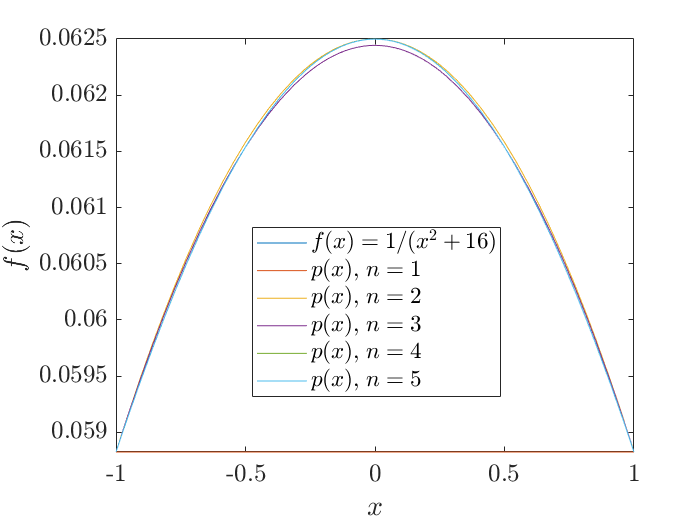
\includegraphics[scale=0.5]{graphics/plot-06.png}
    \caption{Polynomial interpolations of $1 / (x^2 + 16)$ in $[-1, 1]$}
  \end{figure}
\end{solution}